\chapter{Introduction au modèle physique }\label{ch:introduction_physique}

\section{Les piliers}

L'intégralité de l'astrophysique repose sur 3 piliers:
\begin{enumerate}
\item L'observation
\item La théorie
\item La simulation
\end{enumerate}

lien avec la méthode scientifique de manière générale. observation, modélisation et test de la théorie or en astro on ne peut pas tester directement donc on simule.

L'observation est le premier de ces pilier. 
Il est le plus ancien et celui sur lequel repose le plus de poids.
L'Homme a toujours regardé le ciel.
De plus il est commun a toute les disciplines scientifique.
Il n'est pas de science possible sans observation.
La principale difficulté ici, est que le point de vue que nous avons sur l'Univers est unique. 
Il nous est impossible de le regarder sous un autre angle.

Vient ensuite la théorie.
Lorsque l'on voit ces lumière sur la voute celleste, nous sommes obligé de nous poser la question essentielle de leur provenance.
Cette question mène a l'élaboration de diverse formulation tentant d'expliquer comment (et pourquoi) le ciel s'illumine la nuit.  
Dans le cadre de l'étude de l'univers dans sont ensemble, cette théorie est nommée cosmologie et repose sur des concept mathématiques complexes
Il nous est impossible de d'effectuer des expériences sur l'univers, notre porté d'interaction est bien trop réduite.

Enfin, le dernier pilier : la simulation.
Pilier le plus récent il est sensé palier au problème des deux autres : l'impossibilité de changer de point de vue ou de tester les théories élaborées.
Ici sous entendue la simulation numérique, il est beaucoup plus récente et dépend grandement de la technologie.
C'est celui vers lequel j'ai choisis de me diriger.

\section{observation -> Hubble}

découverte des galaxies\\
découverte de l'expansion de l'univers


\begin{figure}[bth]
        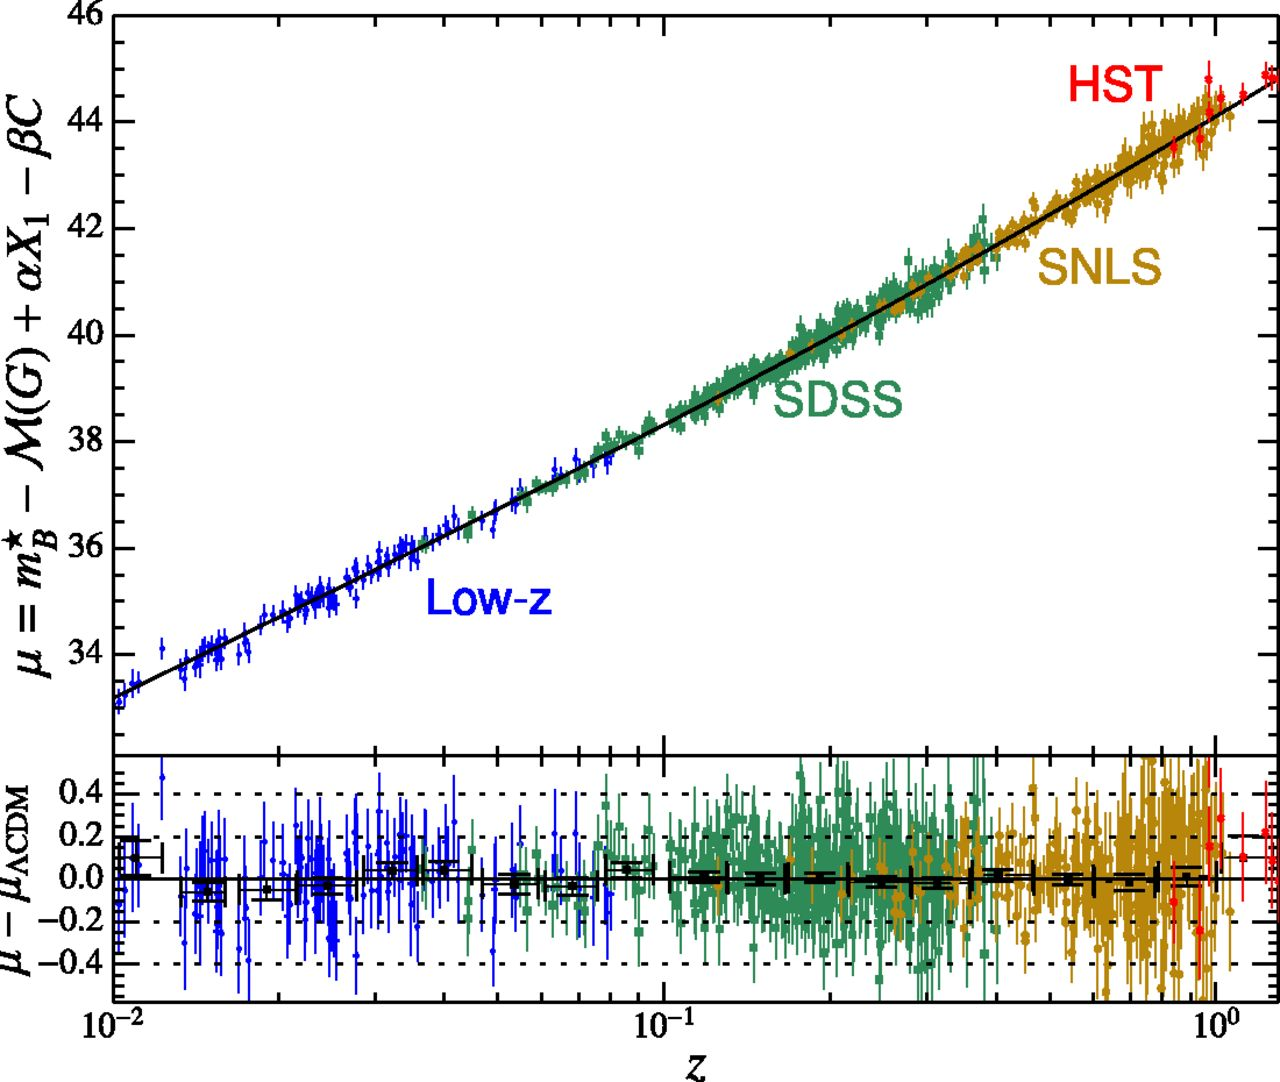
\includegraphics[width=.95\linewidth]{img/01/hubble_law.jpg} 
        \caption{Hubble law. 
%http://www.pnas.org/content/112/11/3173/F2.expansion.html
        Image ESO}
 		\label{fig:hubble_law}
\end{figure}

\begin{equation}
V = H_0 D
\end{equation}


\begin{figure}[bth]
        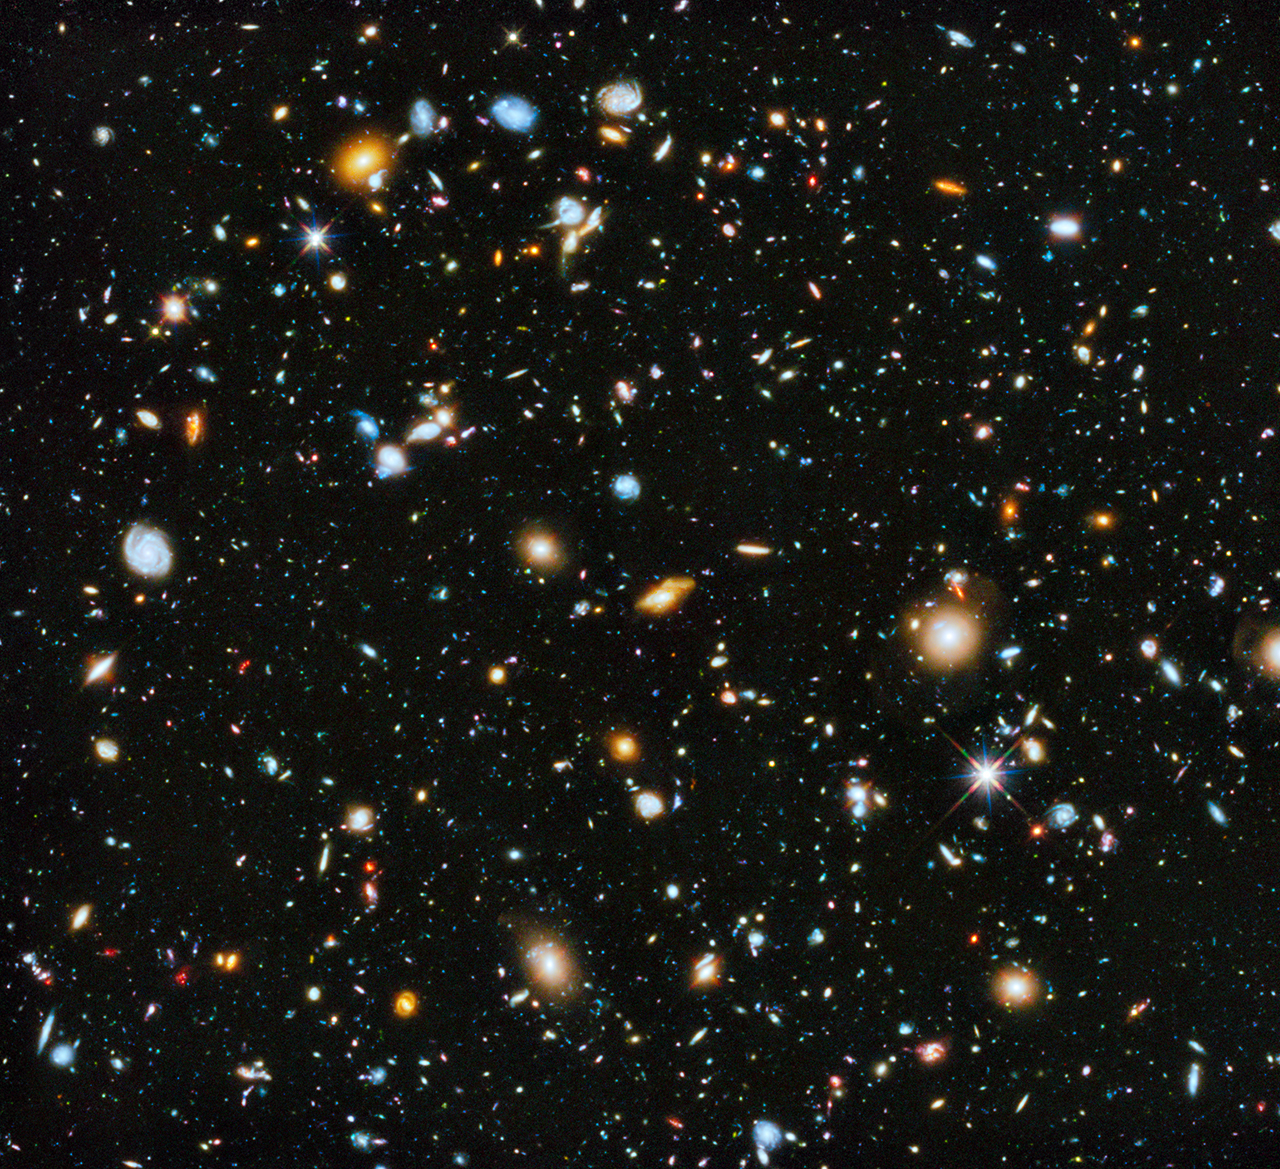
\includegraphics[width=.95\linewidth]{img/01/hudf.jpeg} 
        \caption{Hubble Ultra Deep Field 2014. 
        Image NASA}
 		\label{fig:hubbl_deep_field}
\end{figure}

\section{théorie - lCDM}

le big bang\\
l'inflation\\
la nucléosynthèse\\
le CMB\\
la reionization


\section{Le CMB}


\subsection{Observations}
Penzias et Willson\\

\subsection{Théorie}
surface de dernière diffusion\\


\subsection{Température}
Le cosmic Microwawe background se presente sous la forme du corp noir le plus parfait connus.
Fig. \ref{fig:cmb_thermal_spectrum}
T=2.73K


\begin{figure}[bth]
        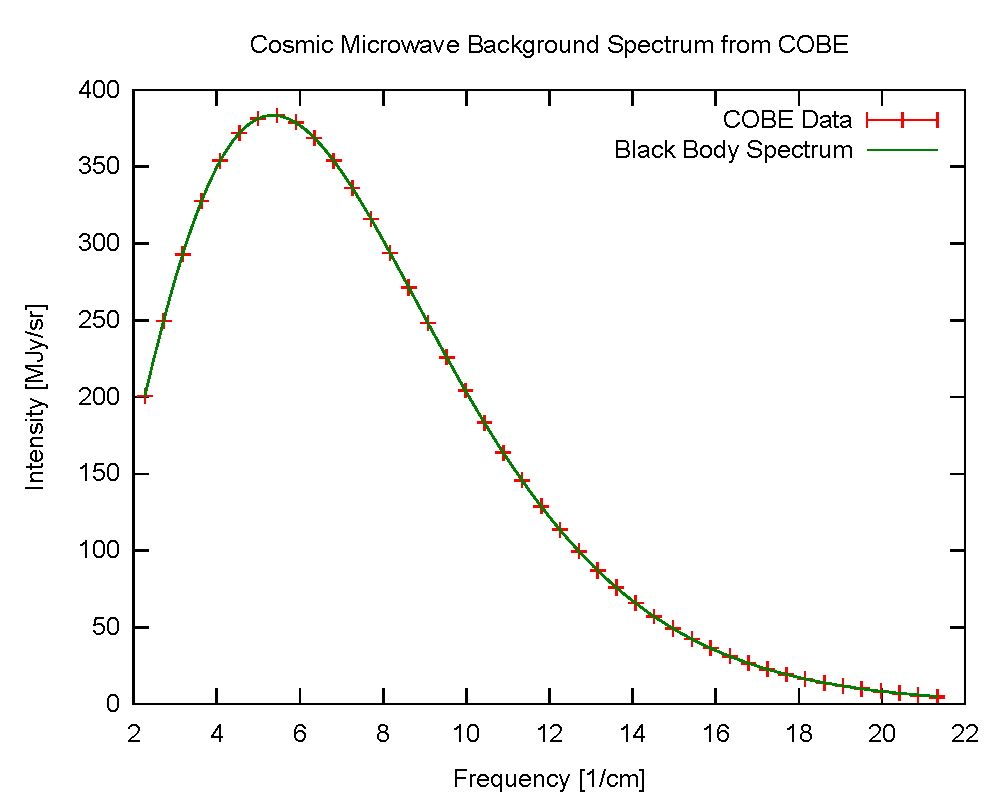
\includegraphics[width=.95\linewidth]{img/01/Cmbr.pdf} 
        \caption{Spectre thermique du CMB vue par le satellite Cosmic Background Explorer (COBE). 
        Image Wikipédia}
 		\label{fig:cmb_thermal_spectrum}
\end{figure}




\subsection{Spectre de puissance}

Le CMB n'est pas uniforme, il presente de tres faibles fluctuations (1e-5)qui nous renseigne sur l'etat de l'univers au moment de son emission.
Fig. \ref{fig:cmb_power_spectrum}

\begin{figure}[bth]
        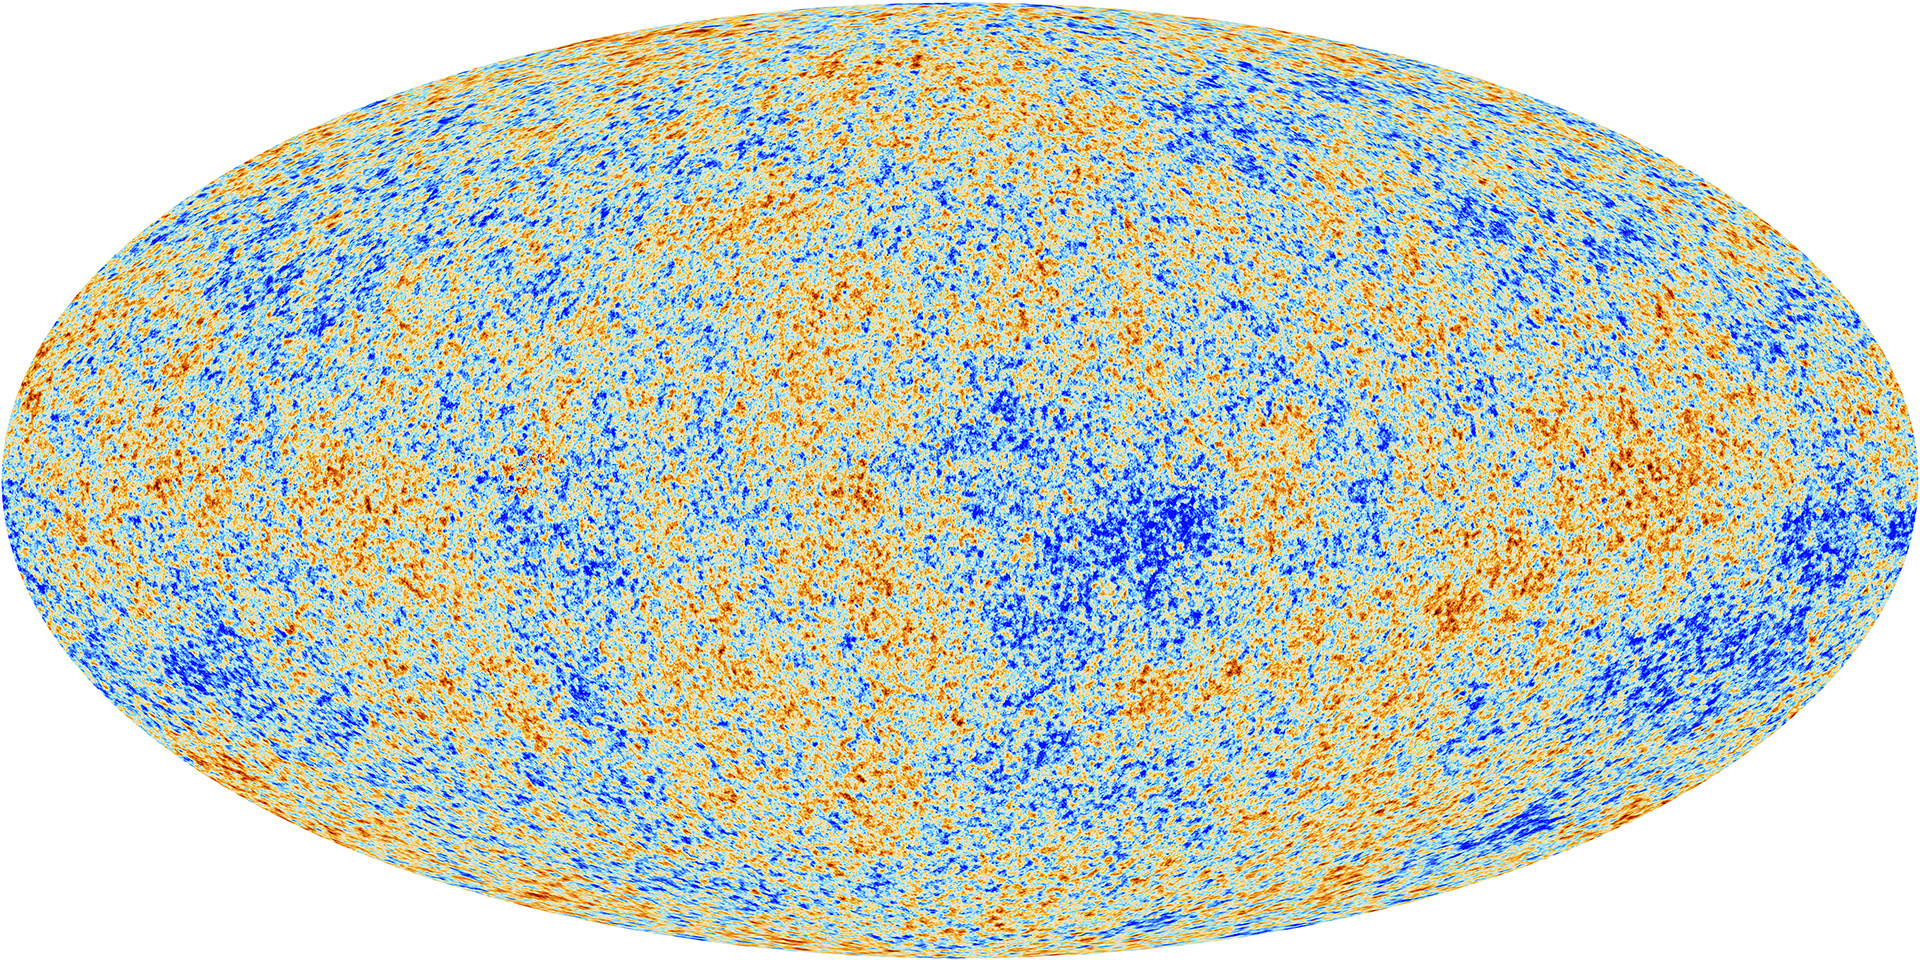
\includegraphics[width=.95\linewidth]{img/01/CMB.jpeg} 
        \caption{Les fluctuation du CMB vues par le satellite Planck. 
        Image ESA}
 		\label{fig:cmb}
\end{figure}


En decomposant ces fluctuations en harmoniques sphériques:
Fig\,\ref{fig:harmoniques_spheriques}

decomposition en multipoles
%https://www.physicsforums.com/threads/can-someone-explain-angular-power-spectrum.309483/
\begin{equation}
 \frac{\Delta T(\theta,\phi)}{T} = \sum_{l>0} \sum_{m=-l}^l a_{lm} Y(\theta,\phi)_{lm}
\end{equation}

avec : 

\begin{equation}
a_{lm}= \int d\Omega(\theta,\phi) \Delta T (\theta,\phi) Y(\theta,\phi)_{lm}
\end{equation}

\begin{figure}[bth]
        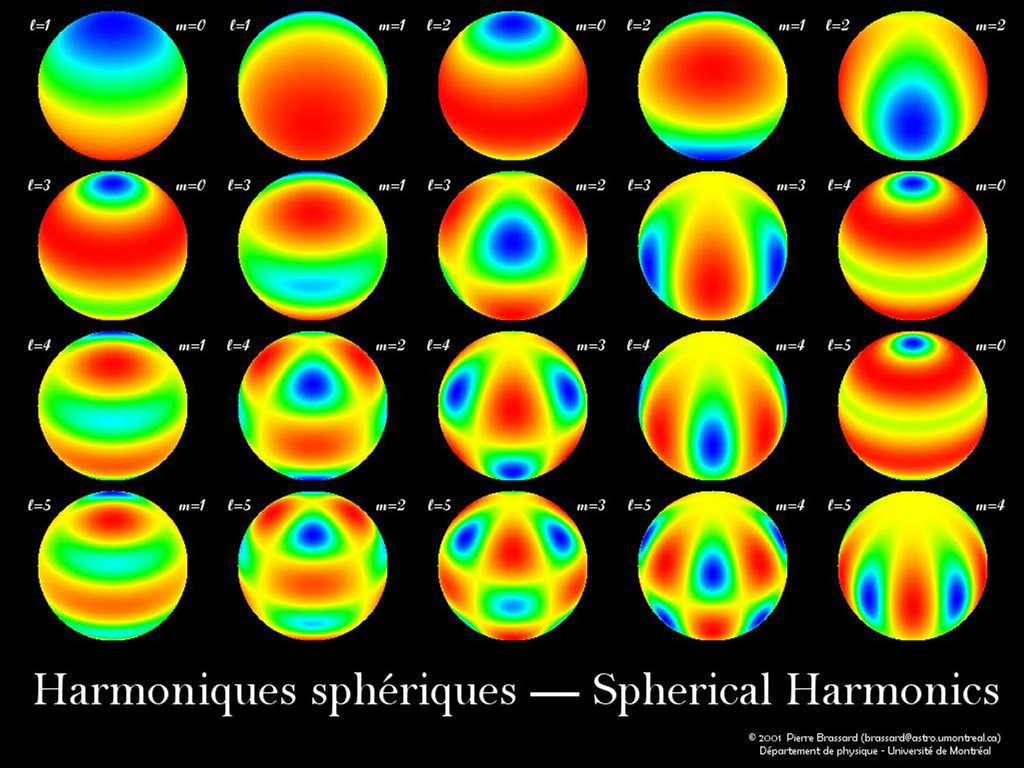
\includegraphics[width=.95\linewidth]{img/01/harmoniques_spheriques.jpeg} 
        \caption{
        représentation des $Y(\theta,\phi)_{lm}$
 Pierre Brassard, université de Montréal 
%Spectre thermique du CMB vue par le satellite Cosmic Background Explorer (COBE). 
        Image Wikipédia}
 		\label{fig:harmoniques_spheriques}
\end{figure}


\begin{equation}
C_l = \frac{1}{2l+1} \sum_{m=-l}^l a_{lm} a_{lm}^*
\end{equation}


Et finalement, on obtient le spectre de puissance:

\begin{equation}
D_l = \frac{l (l+1) C_l }{2 \pi} 
\end{equation}

représenté Fig.\,\ref{fig:cmb_power_spectrum}

\begin{figure}[bth]
        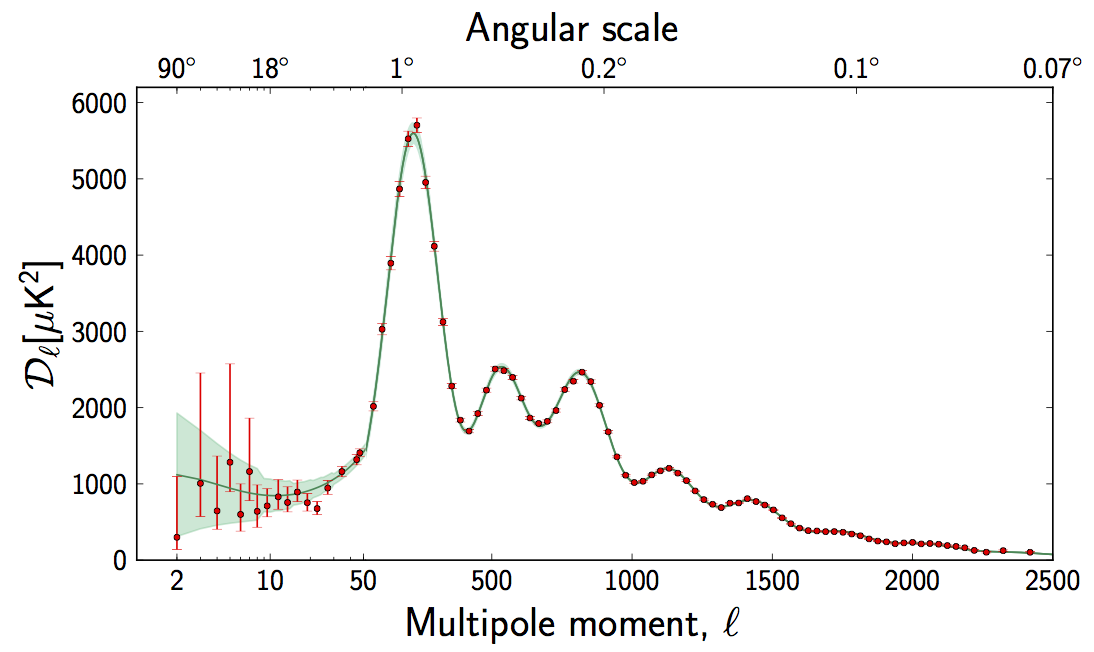
\includegraphics[width=.95\linewidth]{img/01/CMB_power_spectrum.png} 
        \caption{Spectre de puissance des fluctuation du CMB.
        Image ESA}
 		\label{fig:cmb_power_spectrum}
\end{figure}


\section{Le contenu de l'univers - (Théorie)}

Pour simuler l'univers, on a besoin de savoir ce qu'il contient. 
A partir du spectre de puissance, on peut déterminer les différentes composantes de l'univers (paramètres cosmologique).

univers infini, homogène, isotrope


%https://ned.ipac.caltech.edu/level5/Freedman2/Freed6.html


\begin{figure}[bth]
        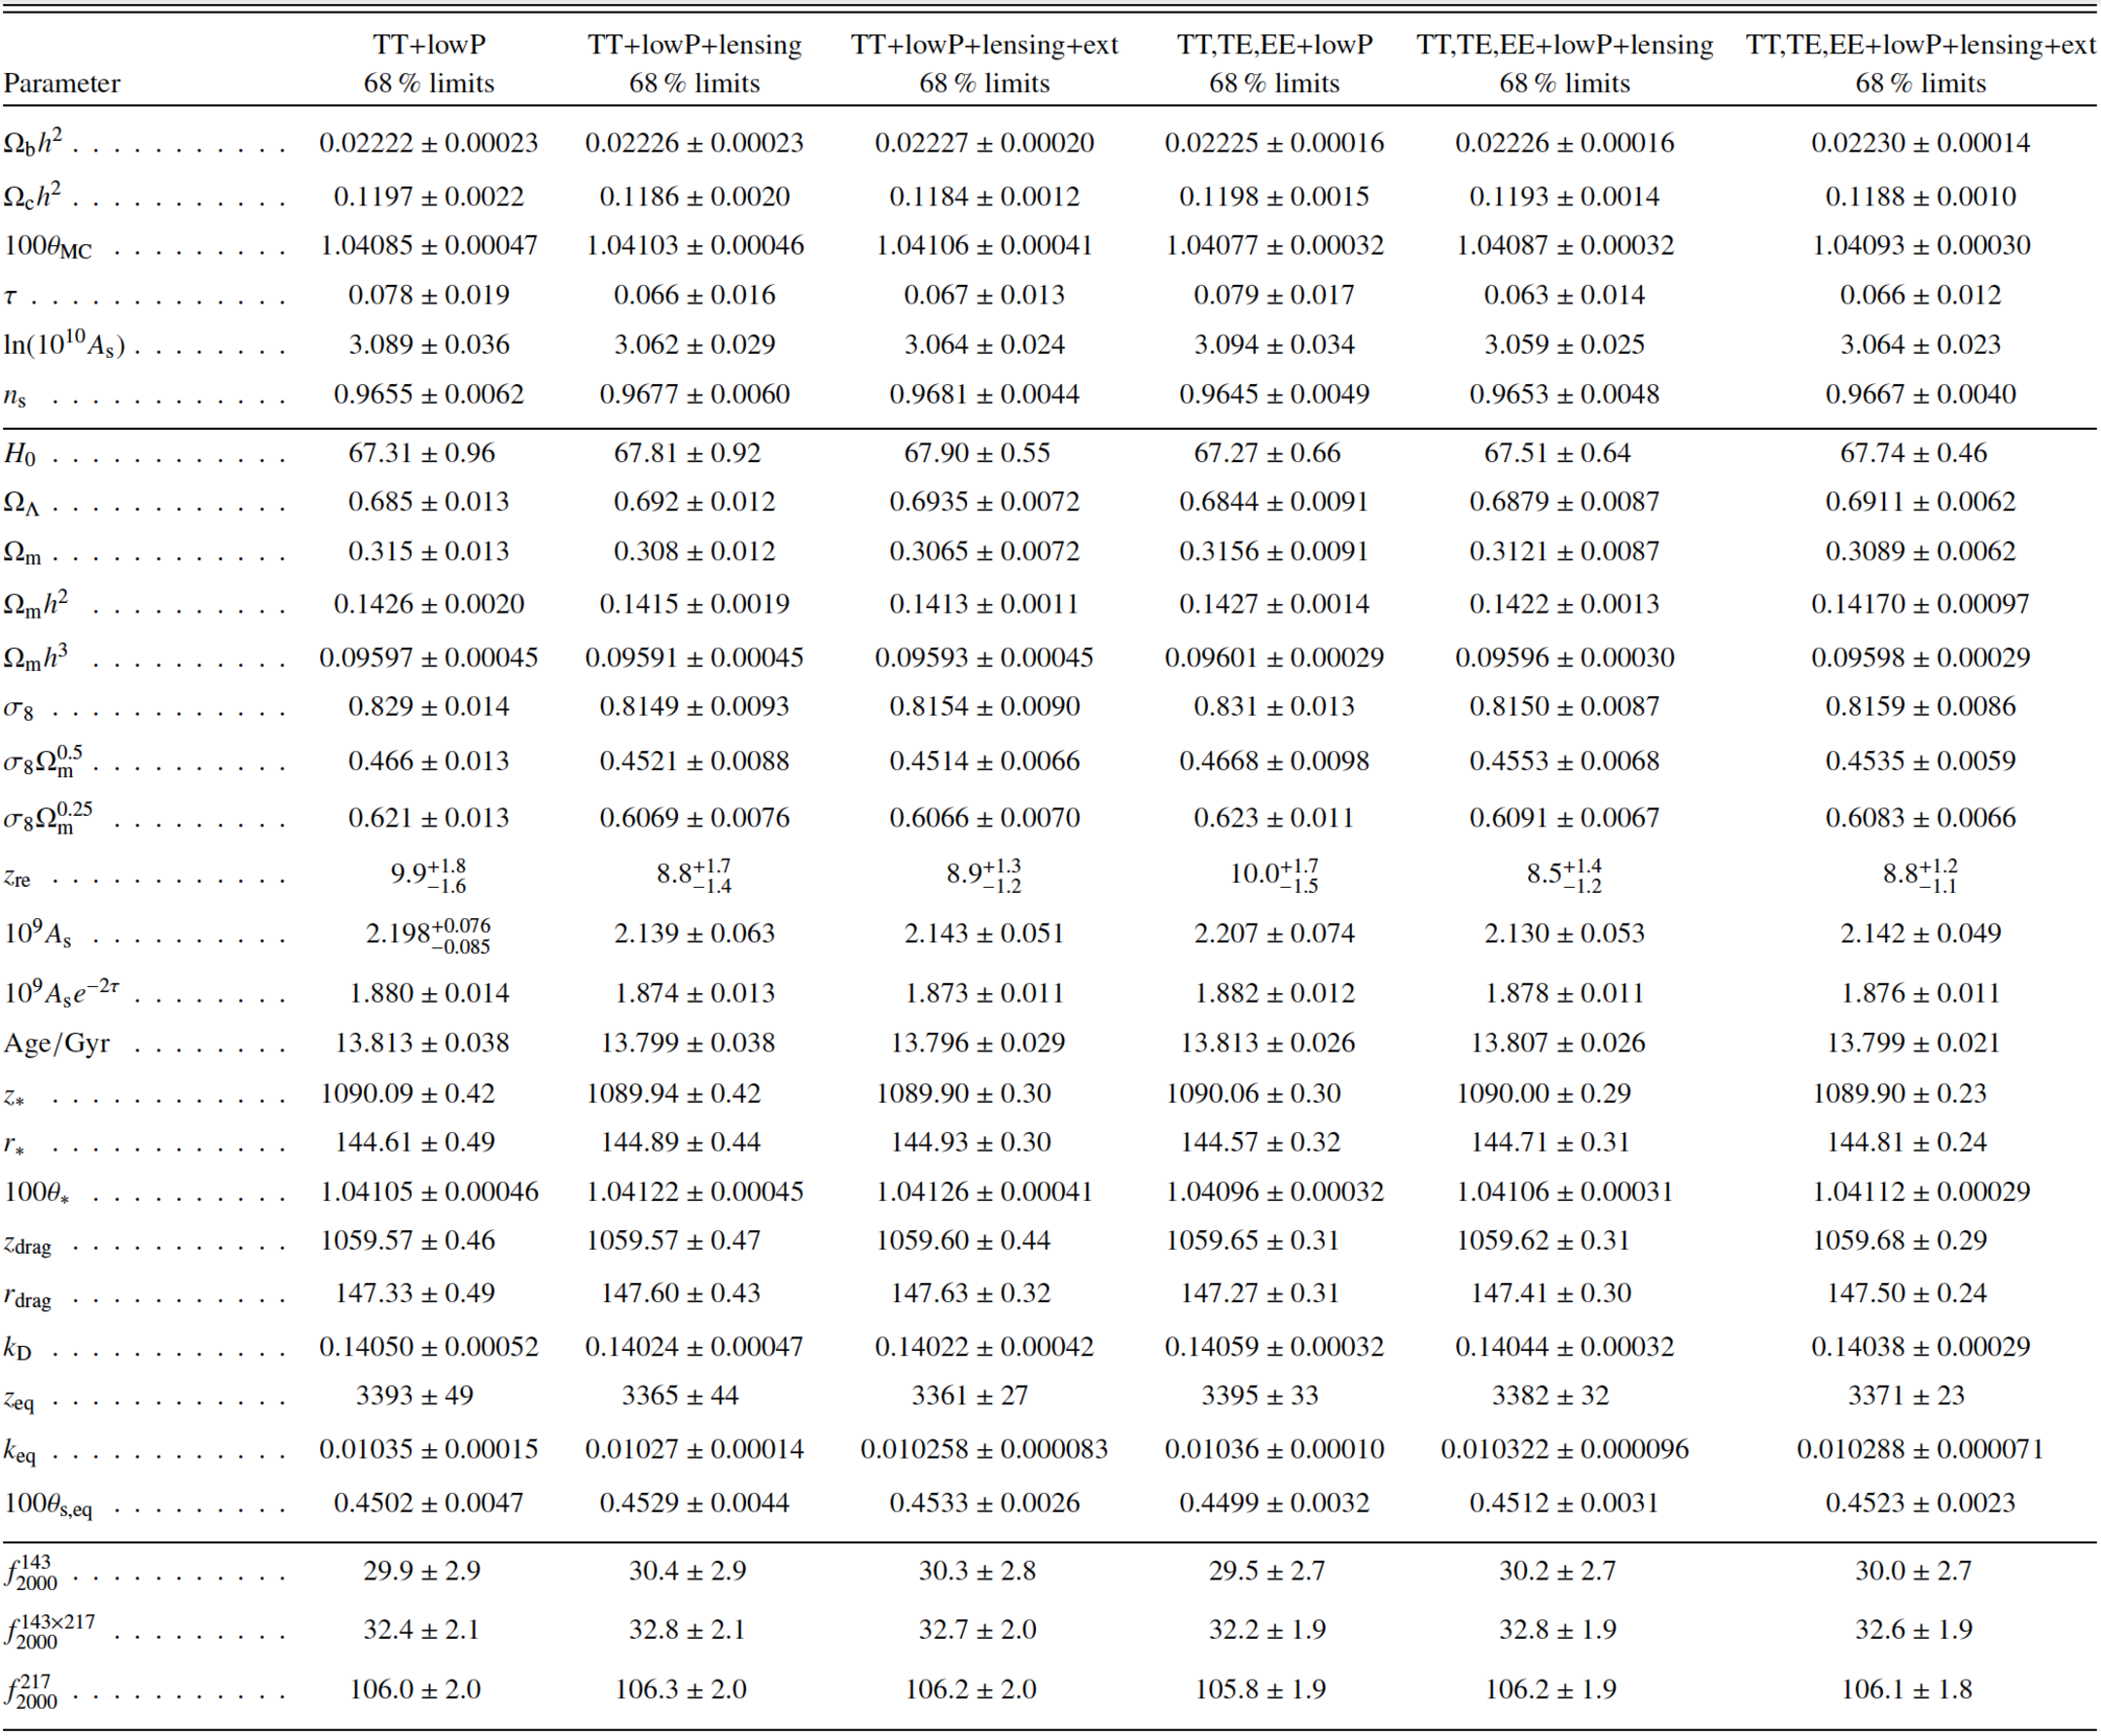
\includegraphics[width=.95\linewidth]{img/01/table_planck.pdf} 
        \caption{Determination des parametres cosmologiques par la colaboration Planck.}
 		\label{fig:planck_parameters}
\end{figure}

\citep{planck_collaboration_planck_2016}

\subsection{Energie noire}

echelle gigaparsec
Facteur d'expansion

\subsection{Matière noire}

echelle mega parsec
gouverne la gravité
non collisionnelle

\subsection{Baryon}

echelle kilo parsec
collisionnelle
interagit avec la radiation
La matière visible

\subsection{Radiation}

quasiment notre seul source d'information sur l'univers (plus vrai depuis les ondes gravitationnelles)
essentielle pour la reionization
seulement E>13.6 eV

\subsection{bilan}

plot en camembert avec les différents constituants

\section{Observation -> la reionization}

le manque d'observations

la difficulté des observations

les futures observations

Quelles sont les preuves de la réionisation?

spectre de quasar\\
tunnel gun peterson
\begin{figure}[bth]
        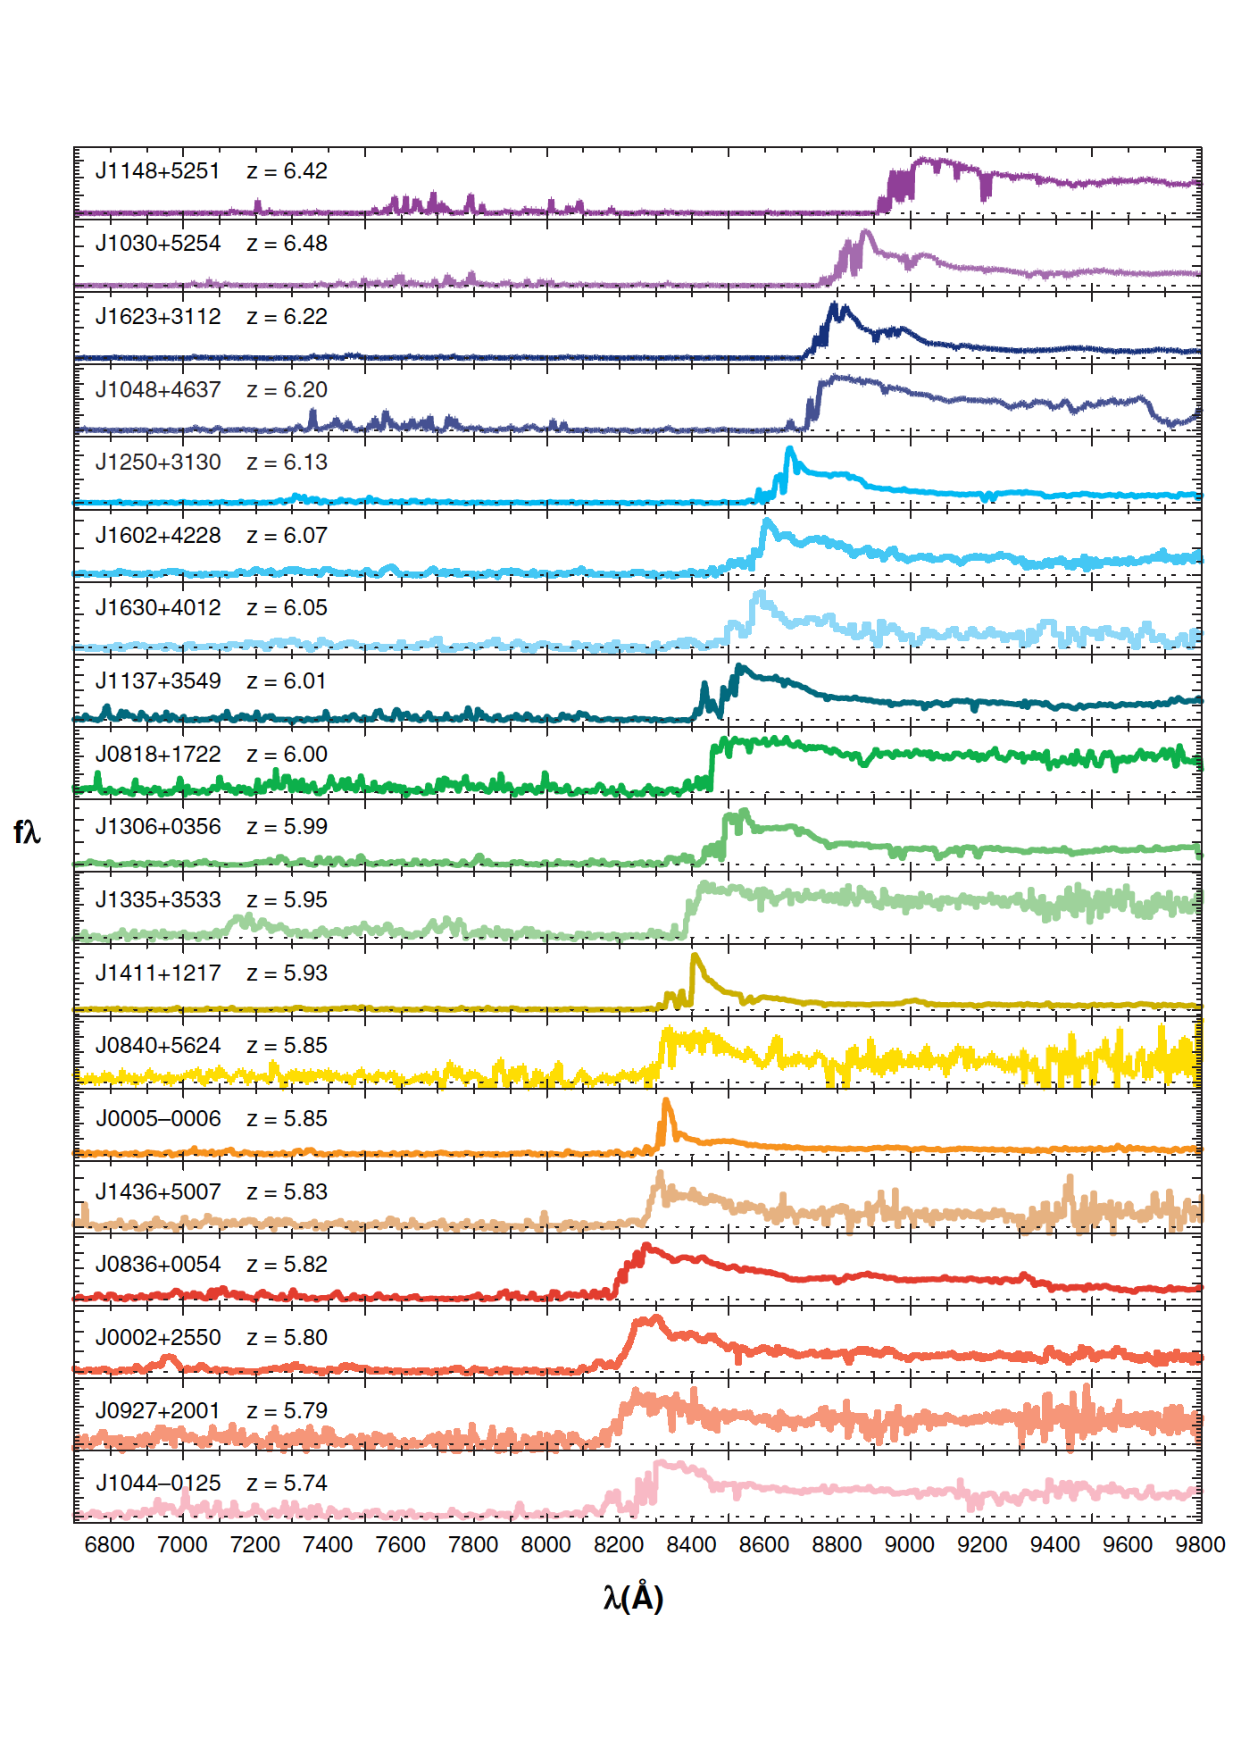
\includegraphics[width=.95\linewidth]{img/01/quasar_spectre.pdf} 
        \caption{Spectre de quasar a differents redshift presentant un tunnel gun peterson.
        Image fan et al.}
 		\label{fig:spectre_quasar}
\end{figure}


polarisation du CMB

ligne 21 cm

fonction de luminosité UV

Epaisseur optique lyman alpha

Epaisseur optique Thomson

\section{Théorie -> La reionization}

réionisation et non rayonnisation!

Qu'est ce que c'est?

fin des âges sombres
apparition des première sources de rayonnement
Pourquoi étudier la réionisation

Dernier processus impactant l'ensemble de l'univers.
Importance pour le "missing satellite problem"

\subsection{les principales question en suspend de l'étude de la réionisation}

quand est ce arrivé?
quelles sont les sources? -> débat galaxies vs quasars
outlier dans l'épaisseur optique des quasars
Le groupe local ?


